%%%%%%%%%%%%%%%%%%%%%%%%%%%%%%%%%%%%%%%%%
% Presentation Template
% LaTeX Template
% Version 2.0 (2023-06-16)
%
% This template was adapted by:
% Jonathan Decker (jonathan.decker@uni-goettingen.de)
% From a template made by:
% Julian Kunkel (julian.kunkel@gwdg.de)
%
%%%%%%%%%%%%%%%%%%%%%%%%%%%%%%%%%%%%%%%%%
\documentclass[compress,aspectratio=169]{beamer}

% make sure the theme and config files are on this path
% uncomment the required theme setting
\usepackage[HPS]{assets/beamerConfig}
%\usepackage[GWDG]{assets/beamerConfig}
%\usepackage[DECICE]{assets/beamerConfig}

\addbibresource{ref.bib}
\graphicspath{{.}{assets/}}

% --- document configuration ---
\newcommand{\mytitle}{Github Actions CI}
% Leave empty for no subtitle
\newcommand{\mysubtitle}{}
\newcommand{\myauthor}{Lars Quentin, Valerius Mattfeld, Frederik Hennecke, Daniil Markovichev}
\newcommand{\myauthorurl}{}
\newcommand{\myvenue}{PCST}
% For example, use \today
\newcommand{\mydate}{13.06.2024}
% For example, Institute for Computer Science / GWDG
\newcommand{\myinstitute}{Ifi}

\configuretitlepage

\begin{document}

	\begin{frame}[plain]
		\titlepage
	\end{frame}

	\begin{frame}[t]{Table of contents}
		\tableofcontents[subsectionstyle=hide/hide]
	\end{frame}

	% --- slides begin ---

	\section{Introduction}

	\begin{frame}{Github Actions}
    \begin{columns}
      \begin{column}{0.5\textwidth}
        \begin{figure}
          \begin{center}
            
\includegraphics[width=0.95\textwidth]{ghlogo.png}
          \end{center}
        \end{figure}
      \end{column}
      \begin{column}{0.5\textwidth}
        \begin{itemize}
          \item CI system developed by Github
          \item Fully hosted, including runner
          \item Uses yaml based configuration
          \item Well documented
          \item Community-driven plugins, so-called "actions"
            \begin{itemize}
              \item integrated marketplace
            \end{itemize}
        \end{itemize}
      \end{column}
    \end{columns}
	\end{frame}

  % Advantages and disadvantages
	\begin{frame}{}
    \begin{columns}
      \begin{column}{0.5\textwidth}
        \begin{block}{Advantages}
          \begin{itemize}
            \item Well documented
            \item Known by many developers
            \item Premade actions for almost everything
            \item No hosting required
            \item Free for non-commercial open source
          \end{itemize}
        \end{block}
      \end{column}
      \begin{column}{0.5\textwidth}
        \begin{block}{Disadvantages}
          \begin{itemize}
            \item Vendor lockin
              \begin{itemize}
                \item Closed source runner
                \item pre made options only available on github
              \end{itemize}
            \item High pricing for large scale
            \item Requires code to be hosted on Github
            \item Runner runs on Github servers
              \begin{itemize}
                \item Possible compliance problems (GDPR)
                \item US Company $\Rightarrow$ CLOUD Act
              \end{itemize}
          \end{itemize}
        \end{block}
      \end{column}
    \end{columns}
	\end{frame}

  \section{Implementation}

  % High Level workflow
	\begin{frame}{High Level Workflow}
    \begin{enumerate}
      \item Create yml file
        \begin{itemize}
          \item \texttt{mkdir -p .github/workflows}
          \item \texttt{touch .github/workflows/ci.yml}
        \end{itemize}
      \item Define when to run
      \item define jobs with different steps. Including:
        \begin{itemize}
          \item Checking out (getting) the code 
          \item Setting up the Environment
          \item The actual work
        \end{itemize}
    \end{enumerate}
	\end{frame}

	\begin{frame}{Config Breakdown: When to Run}
    \begin{columns}
      \begin{column}{0.5\textwidth}
        \begin{figure}
          \begin{center}
            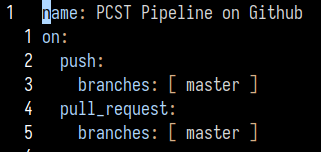
\includegraphics[width=0.95\textwidth]{when.png}
          \end{center}
        \end{figure}
      \end{column}
      \begin{column}{0.5\textwidth}
        \begin{itemize}
          \item Defined by \texttt{on:}
          \item in our case:
          \begin{itemize}
            \item On every master commit
            \item On every pull request against master
          \end{itemize}
        \item Is a list, can contain multiple branches
        \end{itemize}
      \end{column}
    \end{columns}
	\end{frame}

  % each step
	\begin{frame}{Config Breakdown: Build Job}
    \begin{columns}
      \begin{column}{0.5\textwidth}
        \begin{figure}
          \begin{center}
            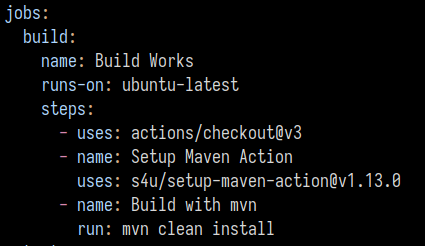
\includegraphics[width=0.95\textwidth]{build.png}
          \end{center}
        \end{figure}
      \end{column}
      \begin{column}{0.5\textwidth}
        \begin{itemize}
          \item Each bullet point is a step that runs one after another
          \item \texttt{actions/checkout} is a pre-made action by Github
            \begin{itemize}
              \item git checkouts the newest version of the repo
            \end{itemize}
          \item \texttt{s4u/setup-maven-action} is a community action to install maven
          \item \texttt{run:} allows for arbitrary shell code execution
        \end{itemize}
      \end{column}
    \end{columns}
	\end{frame}

	\begin{frame}{Config Breakdown: Test Job}
    \begin{columns}
      \begin{column}{0.5\textwidth}
        \begin{figure}
          \begin{center}
            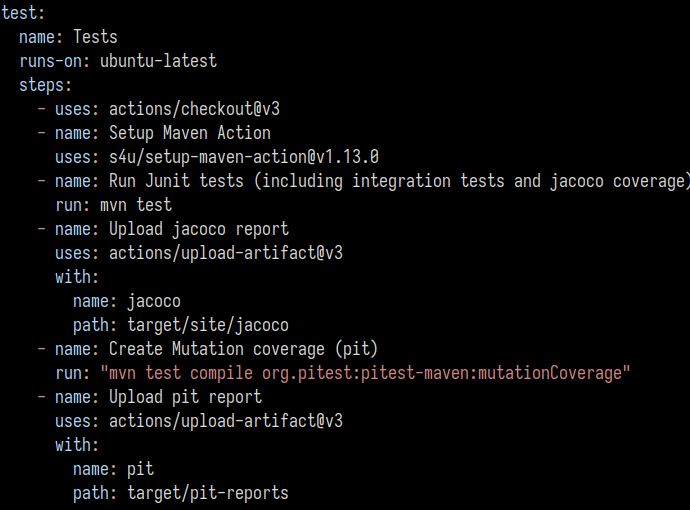
\includegraphics[width=0.95\textwidth]{testjob.png}
          \end{center}
        \end{figure}
      \end{column}
      \begin{column}{0.5\textwidth}
        \begin{itemize}
          \item Again: Checkout and Maven setup
          \item Run unit and integration test suite
            \begin{itemize}
              \item Like in Terminal: \texttt{mvn test}
            \end{itemize}
          \item Run Mutation test coverage with terminal command
          \item \texttt{actions/upload-artifact} is official action by GitHub
            \begin{itemize}
              \item \texttt{with:} can be used to configure actions
              \item \texttt{name:} defines name of the zip file
              \item \texttt{path:} defines where the to-be-zipped files are located
            \end{itemize}
        \end{itemize}
      \end{column}
    \end{columns}
	\end{frame}

	\begin{frame}{Artifacts}
    \begin{figure}
      \begin{center}
        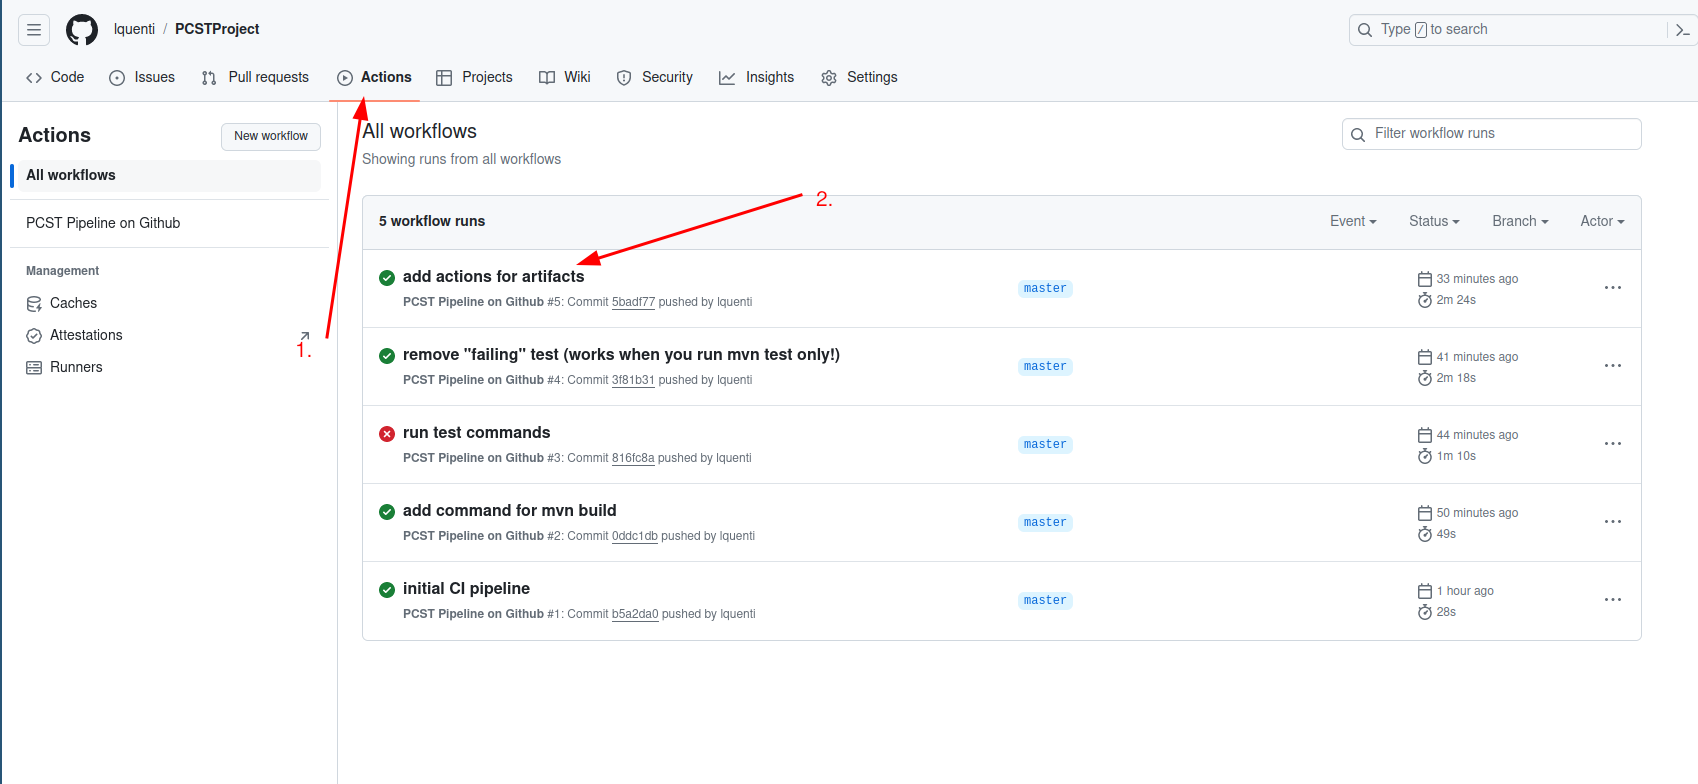
\includegraphics[width=0.95\textwidth]{artifacts1.png}
      \end{center}
    \end{figure}
	\end{frame}
	\begin{frame}{Artifacts}
    \begin{figure}
      \begin{center}
        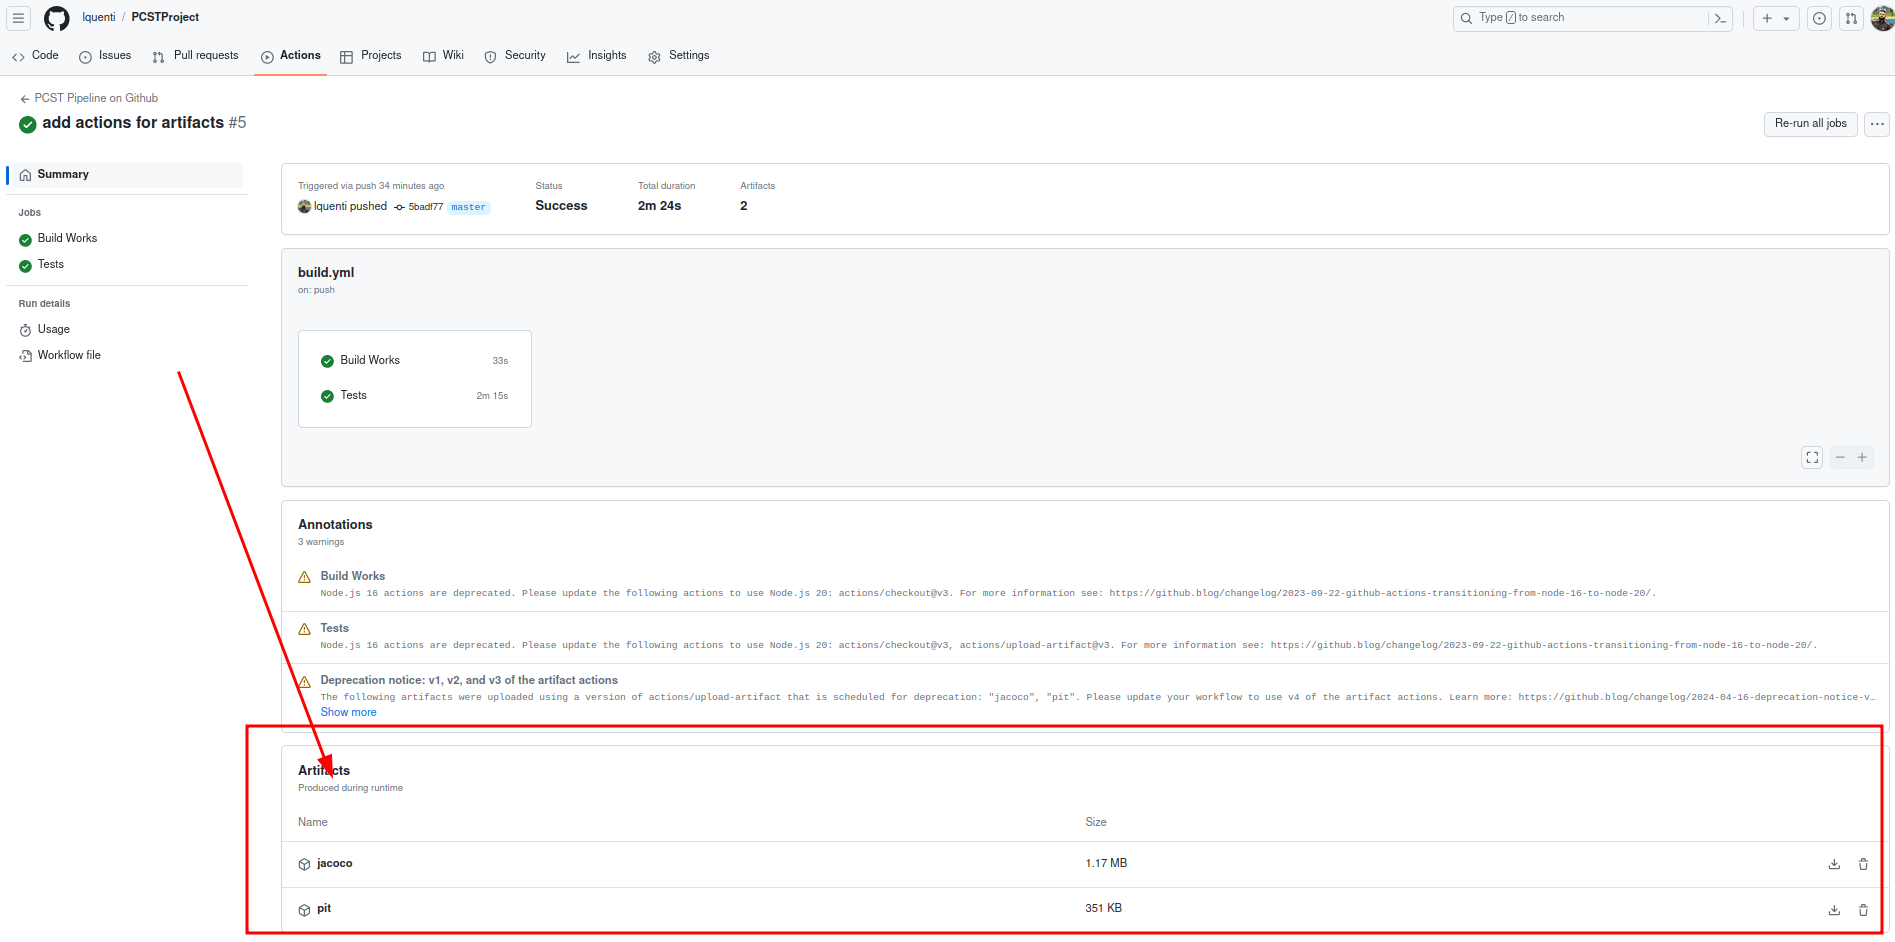
\includegraphics[width=0.95\textwidth]{artifacts2.png}
      \end{center}
    \end{figure}
	\end{frame}
	\begin{frame}{Artifacts}
    \begin{figure}
      \begin{center}
        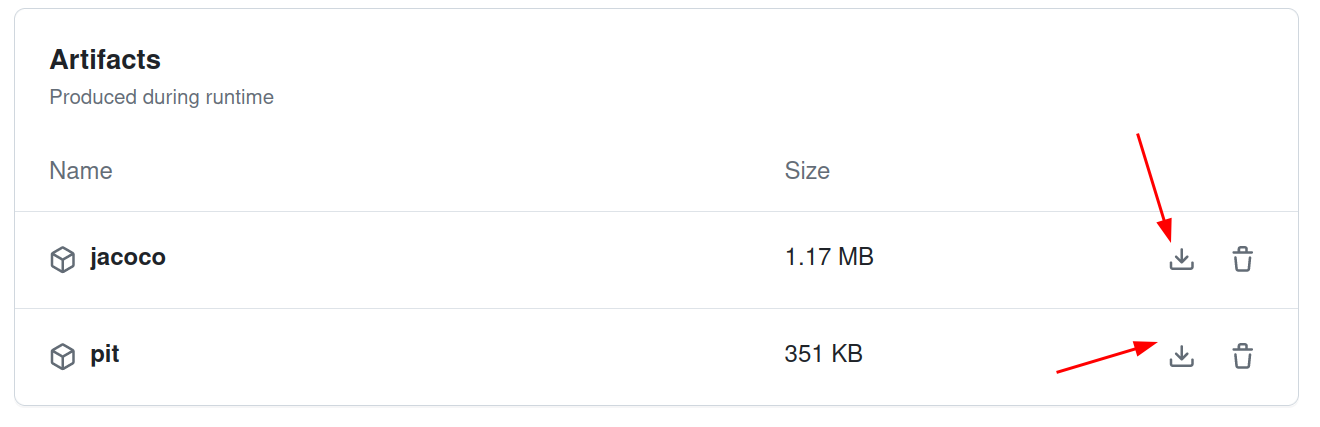
\includegraphics[width=0.95\textwidth]{artifacts3.png}
      \end{center}
    \end{figure}
	\end{frame}

 	\begin{frame}{PIT+Integration tests}
    \begin{columns}
      \begin{column}{0.5\textwidth}
        \begin{figure}
          \begin{center}
            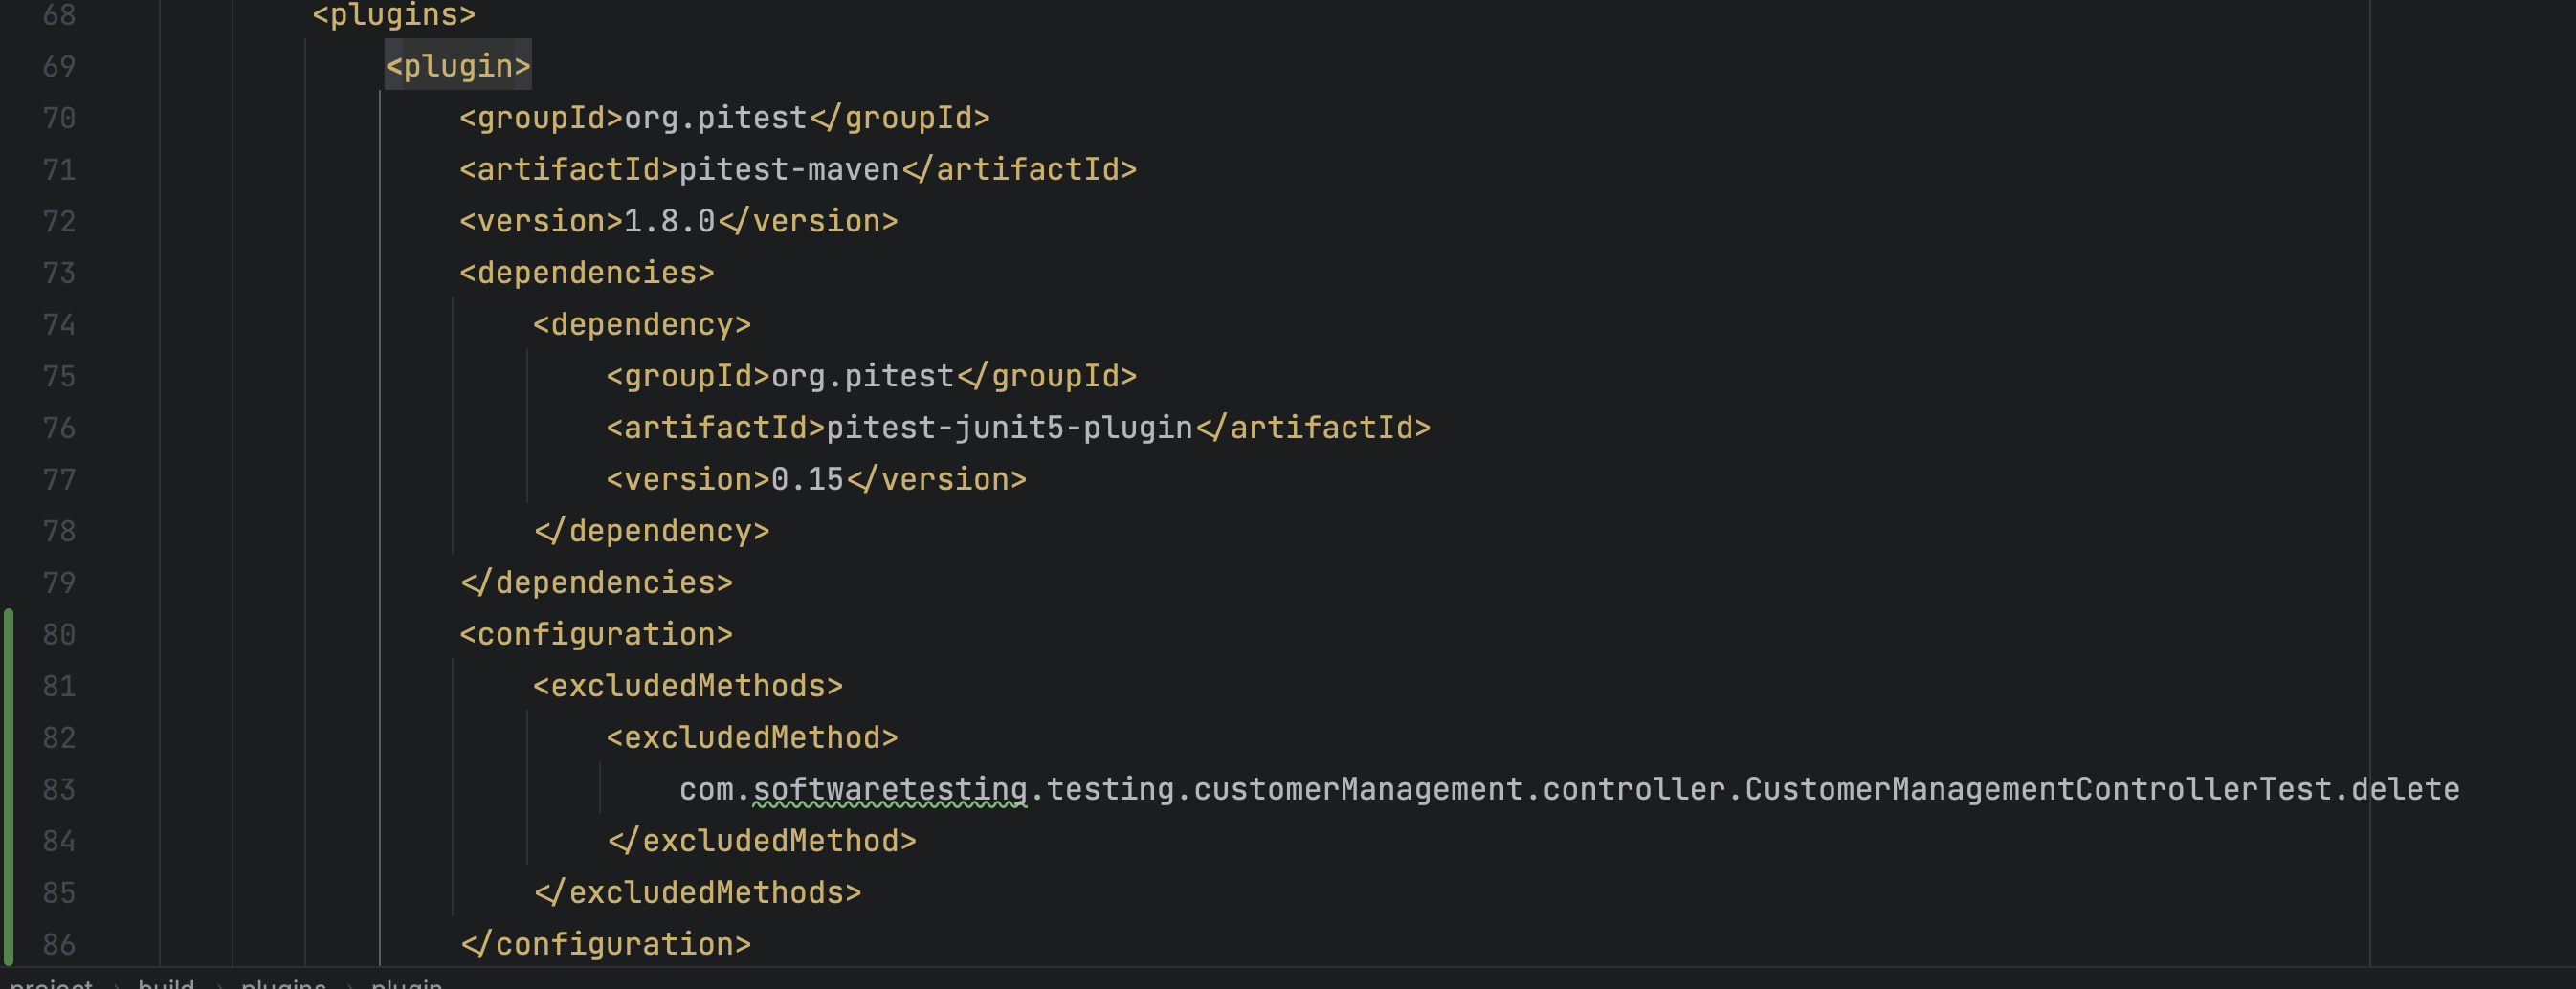
\includegraphics[width=0.95\textwidth]{excludedmethod.png}
          \end{center}
        \end{figure}
      \end{column}
      \begin{column}{0.5\textwidth}
        \begin{itemize}
                \item Integration tests work with \texttt{mvn test}, but not with PIT
                \item There is allegedly a feature to exclude tests with 100\% coverage and 100\% passing
                \item It is not well-documented, so instead the tests were just commented out for now
        \end{itemize}
      \end{column}
    \end{columns}
	\end{frame}

	\begin{frame}{}
		\label{pg:lastpage} % Label on last frame to get the page number for footer
    \begin{center}
    \Huge Thanks for your attention!
    \end{center}
	\end{frame}

\end{document}
